
\section{Results}
\label{sec:results}

\begin{figure*}
    \centering
    \begin{subfigure}[t]{0.5\textwidth}
        \centering
        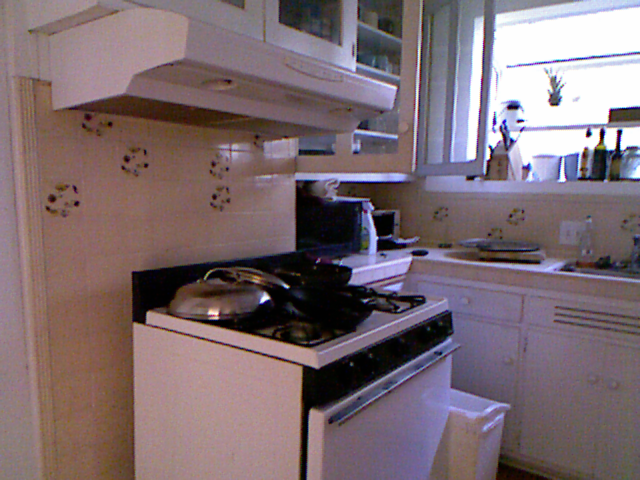
\includegraphics[height=.7\textwidth]{figs/Original321.png}
        \caption{Color}
        \label{fig:original:color}
    \end{subfigure}%
    ~ 
    \begin{subfigure}[t]{0.5\textwidth}
        \centering
        
\includegraphics[height=.7\textwidth]{figs/Depth321.png}
        \caption{Depth (in greyscale)}
        \label{fig:original:depth}
    \end{subfigure}
    \caption{A kitchen scene featuring a stove, oven hood, and cabinets \cite{kinect}.}
    \label{fig:original}
\end{figure*}

\begin{figure*}
    \centering
    \begin{subfigure}[t]{0.33\textwidth}
        \centering
        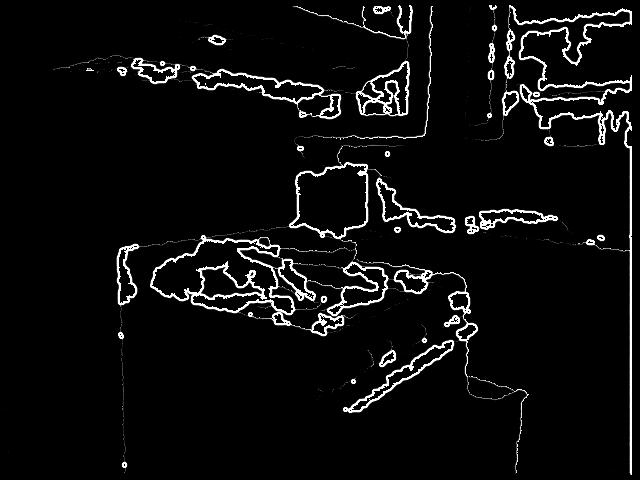
\includegraphics[height=.6\textwidth]{figs/Edged321.png}
        \caption{Edged}
        \label{fig:results:edged}
    \end{subfigure}%
    ~ 
    \begin{subfigure}[t]{0.33\textwidth}
        \centering
        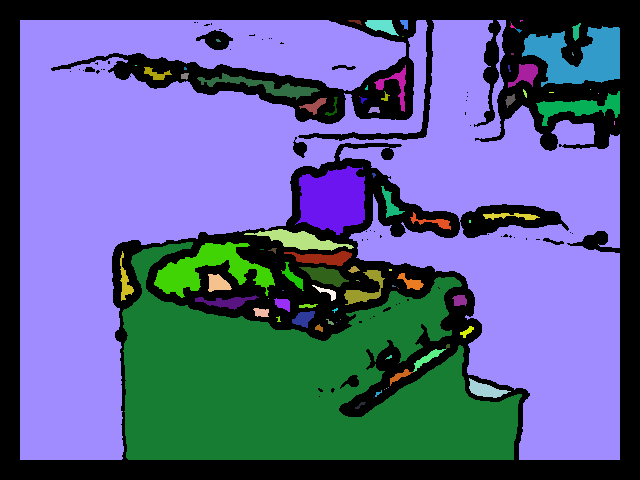
\includegraphics[height=.6\textwidth]{figs/Laplacian321.png}
        \caption{Laplacian Edge Detection}
        \label{fig:results:laplacian}
    \end{subfigure}%
    ~ 
    \begin{subfigure}[t]{0.33\textwidth}
        \centering
        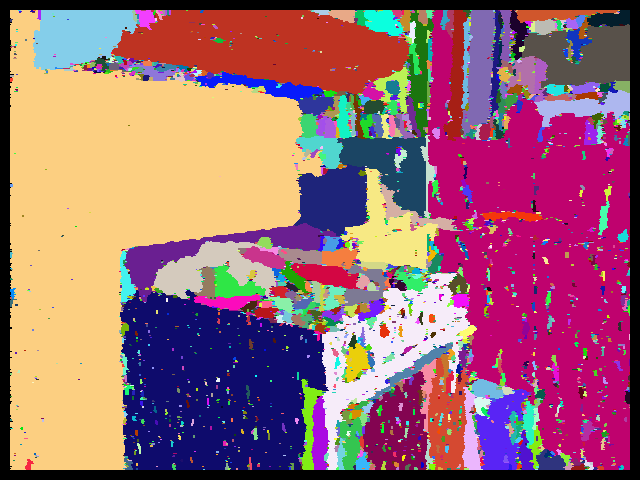
\includegraphics[height=.6\textwidth]{figs/Gradient321.png}
        \caption{Gradient Surface Detection}
        \label{fig:results:gradient}
    \end{subfigure}
    \caption{The segmentation of Fig.~\ref{fig:original:depth} using the Laplacian and Gradient algorithms.}
    \label{fig:results}
\end{figure*}

The fundamental difference in the detection techniques between the algorithms has a highly noticeable effect.  Because Laplacian Edge Detection is sensitive to jump discontinuities, edges of objects and surfaces go unnoticed if they coincide with the edge of another surface, such as on corners.  This effect is visible in  Fig.~\ref{fig:results:laplacian}, where the stove in the center of the image has been correctly segmented, but the front-facing corner of the stove is not reflected in the segmented image.  The jump discontinuities at the back edges of the stove separate it from the wall and cabinets sufficiently to register as a distinct object.

Gradient Surface Detection, on the other hand, reliably detects corners and surface edges.  The faces of the stove are clearly visible in Fig.~\ref{fig:results:gradient}, and sufficient difference in normal vector exists between the wall and the edges of the stove to separate the two into separate regions, like in Fig.~\ref{fig:results:laplacian}.  

It is important to note that reliable behavior for these algorithms was hard to find.  Different images required tuning to see meaningful results, and the Gradient Edge Detection algorithm in general required a cleaning algorithm to partially handle the speckling problem visible in Fig.~\ref{fig:results:gradient}.  We believe this behavior occurs due to random flaws in image quality -- the result of using a realistic data set.